\documentclass[12pt]{article}

\usepackage{minted}
\setminted{fontsize=\small}
\usepackage{sbc-template}
\usepackage{graphicx,url}
\usepackage[utf8]{inputenc}
\usepackage[brazil]{babel}
\usepackage{hyperref}
\usepackage{subfigure}
\usepackage{float}

\sloppy

\title{Reestruturação e aperfeiçoamento de uma ferramenta para detecção de conflitos semânticos de código}

\author{João Pedro Henrique Santos Duarte\inst{1}}

\address{Centro de Informática – Universidade Federal de Pernambuco (UFPE)\\
  Caixa Postal 7.851 –- 50.732-970 –- Recife –- PE -- Brazil
  \email{jphsd@cin.ufpe.br}
}

\begin{document}

\maketitle

\begin{abstract}
In software development, in order to maximize collaboration and parallelize development, it is common to use branches which are later integrated through merges. One of the main problems in this integration are merge conflicts, which negatively affect the project due to the cost involved in its resolution. Although there are tools capable of detecting textual conflicts, semantic conflicts - where changes in software behavior occur - still lack efficient detection tools. The present work proposes to enhance a semantic conflict detection tool based on automated tests, as well as restructure and improve overall code quality of it.
\end{abstract}
     
\begin{resumo} 
No desenvolvimento de \textit{software}, a fim de maximizar a colaboração e o desenvolvimento em paralelo, é comum a utilização de branches que são posteriormente integradas através de merges. Um dos principais problemas nesta integração são os conflitos de merge, que afetam o projeto negativamente pelo custo envolvido em sua resolução. Embora existam ferramentas capazes de detectar conflitos textuais, conflitos semânticos - onde ocorrem mudanças no comportamento do \textit{software} - ainda carecem de ferramentas eficientes de detecção. O presente trabalho propõe o aperfeiçoamento de uma ferramenta de detecção de conflitos semânticos baseada em testes automatizados, como também uma reestruturação com o objetivo de incrementar a qualidade do código.
\end{resumo}

\section{Introdução}
O desenvolvimento de \textit{software} é um processo essencialmente colaborativo. Em diversos projetos, as tarefas são distribuídas entre os desenvolvedores, que trabalham utilizando o conceito de \textit{branches}. \textit{Branches} permitem que a implementação de diferentes funcionalidades do \textit{software} sejam realizadas de maneira independente sendo posteriormente integradas através de processos de \textit{merge}.

Embora esta alternativa facilite o gerenciamento do projeto, \textit{branches} e \textit{merges} trazem com si o surgimento de conflitos de \textit{merge}, que ocorrem durante o processo de integração das modificações de duas \textit{branches} distintas. Alguns destes conflitos já são detectados por ferramentas existentes atualmente, entretanto, especialmente na ocasião dos conflitos semânticos em tempo de execução - onde mudanças realizadas em diferentes partes do \textit{software} acabam resultando em um comportamento diferente em tempo de execução - ainda carecem de ferramentas eficientes de detecção \cite{cavalcanti:icse}.

\cite{leuson:icsme} propõe a ferramenta SMAT, que realiza a detecção de conflitos semânticos por meio da observação automática de mudanças de comportamento entre as diferentes versões do \textit{software} presentes no processo de \textit{merge}. Essa detecção é possível graças a utilização de ferramentas que realizam a geração de testes unitários de forma automática, permitindo que especificações parciais de cada versão sejam construídas e posteriormente comparadas a partir de uma heurística proposta pelos autores.

Apesar de resultados positivos já terem sido observados em SMAT, a implementação da ferramenta enfrenta problemas como a baixa modularidade e dificuldade de extensibilidade e manutenção do código fonte, tal como a baixa configurabilidade, não permitindo customizar aspectos importantes da ferramenta, e a dificuldade de reprodução dos experimentos conduzidos pelo caráter não-determinístico presente na ferramenta. O presente trabalho consiste em uma reestruturação e um aperfeiçoamento desta ferramenta, a nível de arquitetura e implementação, visando solucionar as lacunas supracitadas.

Na seção 2, discutimos um pouco mais a respeito dos conceitos teóricos por trás dos conflitos de integração de código e soluções existentes na literatura para a sua detecção. Na seção 3, apresentamos a ferramenta formulada por \cite{leuson:icsme} para detecção de conflitos semânticos, discutindo suas funcionalidades, implementação e apresentando alguns pontos de melhoria. Na seção 4, discutimos como os pontos de melhoria citados previamente foram implementados a fim de aperfeiçoar a ferramenta de \cite{leuson:icsme}. Por fim, na seção 5, apresentamos e discutimos os resultados obtidos, bem como apresentamos possíveis trabalhos futuros.

\section{Conflitos de Integração de Código}
Conforme mencionado previamente, durante o processo de desenvolvimento de \textit{software} é comum que desenvolvedores realizem suas tarefas em paralelo utilizando \textit{branches} que são posteriormente integradas utilizando \textit{merges}.

Um cenário de \textit{merge} é geralmente composto por dois \textit{commits} \textit{parents} que serão integrados, usualmente denominados \textit{Left} e \textit{Right} e um \textit{commit} resultado da integração entre \textit{Left} e \textit{Right}, denominado \textit{Merge}. Além destes \textit{commits}, adicionaremos também a informação do primeiro \textit{commit} ancestral que é comum ao tronco de \textit{Left} e \textit{Right}, aqui denominado \textit{Base} \cite{leuson:tese}.

\begin{figure}[H]
    \centering
    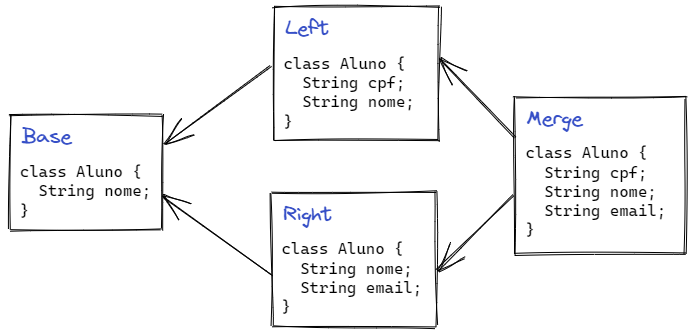
\includegraphics[width=0.80\textwidth]{imagens/merge.png}
    \caption{Visualização simplificada de um cenário de integração de diferentes versões de código. O \textit{commit} \textit{merge} é gerado pela integração das modificações introduzidas em \textit{left} e \textit{right}}
    \label{fig:commits}
\end{figure}

Embora \textit{branches} e \textit{merges} permitam aumentar consideravelmente a produtividade de um time, o processo de integração pode resultar em conflitos, que acabam afetando a produtividade do time - haja vista a deficiência de ferramentas que resolvam estes conflitos automaticamente, como, em casos mais extremos, afetando a corretude do sistema - na ocasião em que os conflitos sequer são detectados \cite{cavalcanti:icse}.

\subsection{Conflitos de merge}
A fim de explorar esta primeira categoria de conflitos, suponhamos o seguinte cenário: dois desenvolvedores, João e Laura, trabalham na mesma equipe de desenvolvimento de \textit{software} para a UFPE. Este projeto possui inicialmente a classe Aluno apresentada na Figura \ref{fig:merge1}.

\begin{figure}[H]
\begin{minted}[linenos]{java}
class Aluno {
  private UUID codigo;
  private String cpf;
  private String email;
}
\end{minted}
\caption{Classe de Aluno presente no projeto.}
\label{fig:merge1}
\end{figure}

Durante uma de suas tarefas, João percebeu que é possível cadastrar um estudante com um email inválido. Em uma nova \textit{branch} denominada \textit{feat-validacao-email}, João decide adicionar um novo método para realizar a validação de um endereço de \textit{email} fornecido chamado \textit{validarEmail(email)}.

Simultaneamente, Laura percebe que um defeito pelo qual ela é responsável é fruto da ausência de validação do CPF. De forma similar ao raciocínio de João, em uma nova \textit{branch} \textit{fix-validacao-cpf}, ela decide também adicionar um método utilitário que realiza a validação do CPF chamado \textit{validarCpf(cpf)}. A Figura \ref{fig:merge2} mostra as diferentes versões do código de João e Laura.
\begin{figure}[H]
\begin{minipage}[t]{0.5\linewidth}
\textbf{João (feat-validacao-email)}\\
\begin{minted}[fontsize=\footnotesize]{java}
class Aluno {
  private UUID codigo;
  private String cpf;
  private String email;

  void validarEmail(String email) {
     (...)
  }
}
\end{minted}
\end{minipage}
\begin{minipage}[t]{0.5\linewidth}
\textbf{Laura (fix-validacao-cpf)}\\
\begin{minted}[fontsize=\footnotesize]{java}
class Aluno {
  private UUID codigo;
  private String cpf;
  private String email;

  void validarCpf(String cpf) {
     (...)
  }
}
\end{minted}
\end{minipage}
\caption{À esquerda, a modificação introduzida por João em sua \textit{branch}. À direita, a modificação introduzida por Laura em sua \textit{branch}}
\label{fig:merge2}
\end{figure}

Ao realizar a integração das modificações de João e Laura, ocorre um conflito de \textit{merge}: ambos os desenvolvedores introduziram modificações diferentes no mesmo trecho de um mesmo arquivo. Este tipo de conflito é detectado pela ferramenta de controle de versão, que altera o arquivo da classe Aluno para reportar a ocorrência do conflito, utilizando uma notação especial, conforme mostra a Figura \ref{fig:merge3}.

\begin{figure}[H]
\begin{minted}[linenos]{java}
class Aluno {
  private UUID codigo;
  private String cpf;
  private String email;

<<<<<<<<<<<<<<
  void validarEmail(String email) {
    (...)
  }
==============
  void validarCpf(String cpf) {
    (...)
  }
>>>>>>>>>>>>>>
}
\end{minted}
\caption{Classe Aluno após a integração das modificações realizadas por João e Laura. As linhas 6, 10 e 14 contém caracteres adicionados automaticamente pelo sistema de gerenciamento de versão para assinalar um conflito de \textit{merge}}
\label{fig:merge3}
\end{figure}

Ainda que este tipo de conflito seja de fácil detecção, a estratégia de \textit{merge} padrão do sistema de controle de versão (merge não-estruturado) não consegue resolvê-lo automaticamente, exigindo uma intervenção manual do desenvolvedor para que o conflito seja solucionado. A literatura propõe a utilização de ferramentas que possuem conhecimento a respeito da linguagem de programação utilizada, para construir \textit{merges} semi-estruturados e estruturados de forma que conflitos semelhantes ao apresentado no exemplo possam ser solucionados sem ser necessária a intervenção do desenvolvedor \cite{cavalcanti:2021}.

\subsection{Conflitos semânticos}
Apesar dos conflitos de \textit{merge} já terem considerável impacto no processo de desenvolvimento, exigindo que um desenvolvedor interrompa suas atividades para resolvê-los, conflitos de integração podem aparecer de diferentes formas, potencialmente causando ainda mais problemas do que os conflitos já discutidos.

Em algumas ocasiões, mesmo que conflitos de \textit{merge} não sejam reportados, o resultado da integração ainda pode resultar em uma versão inválida do \textit{software}, seja por um problema de compilação ou por ter a sua corretude afetada, como ilustrado mais a seguir. Neste trabalho, utilizaremos a nomenclatura adotada por \cite{leuson:tese} para ambos os cenários supracitados, os quais discutimos com mais profundidade nas próximas sessões.

\subsubsection{Conflitos semânticos em tempo de compilação}
A fim de discutir essa categoria de conflitos de integração, suponhamos o seguinte exemplo, ainda dentro do contexto de uma equipe de desenvolvimento de \textit{software} acadêmico na UFPE. Desta vez, João está trabalhando na refatoração de uma classe no projeto responsável por realizar chamadas a uma API externa, cuja implementação inicial é mostrada pela Figura \ref{fig:build1}.

\begin{figure}[H]
\begin{minted}[linenos]{java}
class GovApiService {
   public Student getStudentFromGov(Cpf aCpf) {
      (...)
   }
}
\end{minted}
    \caption{Código Java da versão inicial da classe modificada por João}
    \label{fig:build1}
\end{figure}

Durante a refatoração, João optou por alterar o nome do método \textit{getStudentFromGov} para \textit{fetchStudentFromGov}. Em paralelo e em outra \textit{branch}, Laura está desenvolvendo uma nova funcionalidade que realizará uma chamada à API externa utilizando a classe modificada por João. Por uma falha de comunicação e planejamento, Laura ainda não possui a versão atualizada de João e, portanto, realiza a chamada utilizando o nome \textit{getStudentDataFromGov}.

\begin{figure}[H]
\textbf{João}
\begin{minted}[linenos]{java}
class GovApiService {
 public Student fetchStudentFromGov(Cpf aCpf) {
    (...)
 }
}
\end{minted}
\textbf{\newline Laura}
\begin{minted}[linenos]{java}
class AlunoController {
  public Student createStudent(Cpf aCpf) {
    Student aStudent = govService.getStudentFromGov(aCpf);
    (...)
 }
}
\end{minted}

\caption{Na parte superior, a modificação introduzida por João em um arquivo (a renomeação de um método). Já na parte inferior, a modificação introduzida por Laura em outro arquivo (que envolve uma chamada ao método que foi renomeado por João).
}
\label{fig:build2}
\end{figure}

Ao realizarem a integração deste código, a ferramenta de versionamento de código não reporta nenhum conflito de \textit{merge}, de fato, as mudanças ocorreram em arquivos diferentes. Entretanto, a nova versão resultado da integração de ambas as versões não passa nas checagens de integração contínua do projeto, sendo reportado um erro de compilação do tipo símbolo não-existente, resultado da invocação do método \textit{getStudentFromGov} por \textit{right}, método este, que foi renomeado na classe \textit{GovApiService} em \textit{left}.

Mesmo que, à primeira vista, a situação demonstrada acima possa parecer ter ocorrência rara em ambientes reais de desenvolvimento de \textit{software}, este tipos de conflitos ocorrem com considerável frequência. Além disso, diferentemente dos conflitos de \textit{merge}, que possuem ferramentas maduras para detecção e ferramentas promissoras para a sua solução, conflitos em tempo de compilação geralmente exigem que os próprios desenvolvedores realizem correções manualmente de modo que o \textit{software} seja compilável novamente \cite{leuson:build}, custando tempo e qualidade para o projeto.

\subsubsection{Conflitos semânticos em tempo de execução}
Até aqui, discutimos categorias de conflitos que, apesar de afetarem a produtividade, ainda são detectados durante a etapa de desenvolvimento, inclusive já dispondo de ferramentas que conseguem detectá-los com certa facilidade. Nesta seção, discutiremos uma categoria de conflitos que surgem durante integrações que geram versões compiláveis do \textit{software}, mas que em tempo de execução fornecem resultados diferentes dos esperados.

A fim de compreender como estes conflitos podem ocorrer na prática, tomemos como exemplo a seguinte situação: suponha que dois desenvolvedores estão trabalhando no método de validação de uma determinada classe de forma independente. O código resultado da integração de ambas as contribuições está representado na Figura \ref{fig:dynamic1}.

\begin{figure}[H]
\begin{minted}[linenos]{java}
class Aluno {
   public static void validarAluno(String email) {
      StringUtils.assertMinLength(email, 15);
      (...)
      StringUtils.assertMaxLength(email, 10);
   }
}

\end{minted}
\caption{Código Java resultado da integração entre as versões. A linha 3 é oriunda de uma contribuição de \textit{left}, enquanto a linha 5 é oriunda de \textit{right}.}
\label{fig:dynamic1}
\end{figure}

Observemos a ausência de conflitos de \textit{merge}, de fato, as modificações ocorrem em trechos distintos do código, e que a versão obtida após a integração é compilável, apontando a ausência de conflitos semânticos em tempo de compilação. Todavia, se executarmos o programa resultante, observamos um comportamento diferente do esperado.
	
Analisando as versões a serem integradas de forma isolada, podemos extrair especificações implícitas do comportamento esperado por cada desenvolvedor ao realizar as suas modificações. No exemplo da Figura \ref{fig:dynamic1}, enquanto \textit{left} especifica que o \textit{email} deve ter no mínimo 15 caracteres, \textit{right} especifica que o valor não pode ultrapassar 10 caracteres. Embora estas especificações estejam implementadas corretamente em ambas as versões, a coexistência de ambas é logicamente inconsistente resultando em um programa que lança exceções para entradas que seriam aceitas apenas por \textit{left} ou \textit{right}.

Esta situação aponta a presença de um conflito durante a integração que se manifesta apenas em tempo de execução. Como a detecção desta categoria de conflitos carece de ferramentas automáticas, as últimas barreiras para a detecção destes conflitos em uma equipe é a adoção de boas práticas como a utilização de suítes de testes automatizadas e políticas de revisões de código. Mesmo assim, inclusive projetos que possuem boa cobertura de testes e políticas estritas de revisão correm o risco de negligenciar tais conflitos, permitindo que estes cheguem ao \textit{software} em produção \cite{leuson:tese}.

\subsubsection{Detectando conflitos semânticos em tempo de execução}
Detectar conflitos semânticos em tempo de execução possui elevada dificuldade. De fato, detectar tais conflitos envolveria construir uma ferramenta que fosse capaz de compreender o comportamento esperado do \textit{software}, e o efetivamente implementado em cada um dos \textit{parents} envolvidos na integração, podendo então avaliar a existência de interferências e potenciais conflitos entre cada uma das versões. Entretanto, neste contexto, esta avaliação é um problema que não é sequer computável \cite{cavalcanti:icse}.

Mesmo assim, soluções heurísticas são propostas na literatura, geralmente utilizando ferramentas de análise estática, a fim de detectar tais conflitos. Neste trabalho, focaremos na ferramenta SMAT, proposta por \cite{leuson:icsme}, que utiliza uma estratégia diferente das apresentadas até então.

\section{Ferramenta SMAT} \label{smat}
Conforme apresentado na seção anterior, detectar conflitos semânticos em tempo de execução é um processo difícil e ainda são poucas as propostas de ferramentas capazes de atacar esse problema de forma eficaz. Neste contexto, \cite{leuson:icsme} propõe a ferramenta SMAT que utiliza uma estratégia diferente das utilizadas por outras ferramentas que possuem a mesma finalidade.

Para o método modificado onde se quer investigar a ocorrência de conflitos semânticos, aqui denominado \textbf{método alvo}, SMAT utiliza ferramentas que realizam a geração automática de suítes de testes já propostas na literatura, como \textit{Evosuite} \cite{evosuite:manual} e \textit{Randoop} \cite{randoop}, para construir especificações parciais do método alvo em ambos os \textit{parents}. Como exemplo, suponha o teste da Figura \ref{fig:teste}, que especifica parcialmente a modificação introduzida por \textit{right} no exemplo da seção anterior.

\begin{figure}[H]
\begin{minted}[linenos]{java}
@Test
public void test() {
  Exception e = assertThrows(StringException.class, () -> {
    String email = "12caracteres"; // string com tamanho 12
      Aluno.validarAluno(email);
  });
  assertTrue(e.getMessage()
    .equals("String não pode ter mais que 10 caracteres");
}
\end{minted}
\caption{Caso de teste de exemplo para a modificação introduzida por \textit{right} no exemplo da Figura \ref{fig:dynamic1}}
\label{fig:teste}
\end{figure}
SMAT então realiza comparações destas especificações em cada versão do  \textit{software} através da execução dos casos de teste gerados em cada uma das versões contidas no cenário de \textit{merge}. O resultado da execução dos casos de testes são avaliados com o objetivo de detectar conflitos que atendam aos seguintes critérios heurísticos:
\begin{itemize}
    \item A execução do teste falha em pelo menos um dos \textit{parents} e passa em \textit{Base} e \textit{Merge}. Analogamente, um conflito também é detectado se a execução do teste passa em pelo menos um dos \textit{parents} mas falha em \textit{Base} e \textit{Merge}.
    \item A execução do teste falha em ambos os \textit{parents} e em \textit{Base}, mas passa em \textit{Merge}. Analogamente, um conflito também é detectado se a execução do teste passa em ambos os \textit{parents} e em \textit{Base} mas falha em \textit{Merge}.
\end{itemize}
Como o caso de teste da Figura \ref{fig:teste} passa na versão do código de \textit{right} e falha em \textit{base}, afinal nenhuma validação a respeito do tamanho da \textit{String} é realizada. Embora o teste também falhe em \textit{merge}, a exceção levantada pela validação é pelo fato da \textit{String} de teste possuir comprimento inferior ao permitido, comportamento introduzido por \textit{left}. Este cenário de interferência satisfaz o primeiro critério para detecção de um conflito semântico, sendo então reportado por SMAT ao usuário.

A fim de evitar que testes que tenham comportamento \textit{flaky}, isto é, que não apresentam resultados consistentes ao longo de várias execuções, possam interferir no resultado fornecido pela ferramenta, SMAT realiza 3 execuções de cada caso de teste, descartando-o na análise na presença de qualquer disparidade entre os resultados.

Outra preocupação existente é com testes que venham a falhar por exercitarem elementos que não estão presentes em alguma versão do código que está sendo analisado - suponha, por exemplo, a introdução ou remoção de um método em algum dos \textit{parents}. Neste contexto, a avaliação seria inconclusiva e, portanto, tais testes são descartados durante a análise.

\subsection{Arquitetura e Implementação de SMAT}
A implementação original de SMAT\footnote{\href{https://github.com/spgroup/SMAT/tree/ae33ccdc49}{https://github.com/spgroup/SMAT/tree/ae33ccdc49}} é realizada em \textit{Python} com aproximadamente 3800 linhas de código, e é fruto de um \textit{fork} da ferramenta Nimrod, originalmente utilizada para experimentos com teste de mutação.

A ferramenta pode ser estruturada conceitualmente como sendo composta por 4 módulos que coincidem com as 4 etapas sequenciais da execução de SMAT: geração das suítes de testes \textit{(Test Generation)}, execução destas suítes \textit{(Test Execution)}, análise dos resultados \textit{(Dynamic Analysis)} e geração de relatórios \textit{(Output Generation)}, estruturados arquiteturalmente na aplicação como mostra a Figura \ref{fig:macro-velha}.

\begin{figure}[H]
    \centering
    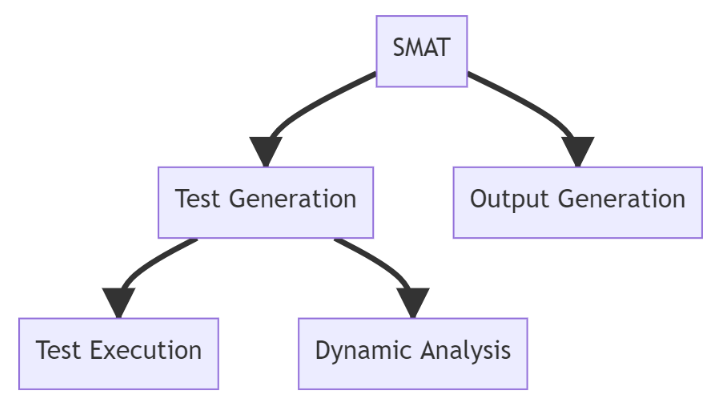
\includegraphics[width=.5\textwidth]{imagens/arquitetura-velha.png}
    \caption{Diagrama da macro-arquitetura de SMAT.}
    \label{fig:macro-velha}
\end{figure}

SMAT recebe como entrada um ou mais cenários de merge dispostos em um arquivo CSV que obedece a seguinte estrutura:

\begin{itemize}
    \item Nome do projeto a ser analisado;
    \item Um booleano indicando se o cenário deve ser analisado ou não;
    \item Seguem 4 colunas com as \textit{hashes} dos \textit{commits} que serão analisados (\textit{base, left, right e merge});
    \item \textit{Fully-Qualified Class Name (FQCN)} da classe alvo. Mais de uma classe pode ser informada utilizado o caractere | como separador;
    \item Assinatura do método alvo. Somente um método pode ser fornecido. Os argumentos do método devem ser informados utilizando o caractere | como separador;
    \item Seguem 4 colunas com o caminho para os JARs de cada SHA (\textit{base, left, right e merge}). Estas versões são necessárias para que sejam informadas ao gerador de testes.
\end{itemize}

\subsection{Limitações e pontos de melhoria de SMAT}
Apesar de SMAT ter apresentado resultados positivos na detecção dos conflitos, tendo sido capaz de detectar corretamente mais de 30\% dos casos presentes na amostra estudada em trabalho anterior \cite{leuson:icsme}, a ferramenta possui algumas limitações e pontos de melhoria relacionados à sua implementação e arquitetura.

Pela natureza exploratória das ferramentas de geração de testes utilizadas, é possível que o método alvo da análise não seja exercitado por nenhum caso de teste que atenda aos critérios heurísticos implementados. Assim, como SMAT não leva em consideração os métodos executados em um caso de teste durante a análise, é possível que um conflito seja reportado sem que o método alvo tenha sido executado, consistindo assim em um falso positivo.

Junto a isto, SMAT possui a limitação de conseguir analisar apenas um único alvo por execução. Por exemplo, se no cenário da seção anterior estivéssemos interessados em executar a análise para outro método, teríamos que realizar uma nova chamada a SMAT e, por consequência, realizar uma nova chamada as ferramentas geradoras de testes e novas chamadas a execução dos testes, o que aumentaria consideravelmente o tempo de execução da ferramenta.

Do ponto de vista arquitetural, embora as 4 etapas da execução possuam um isolamento conceitual, a atual hierarquia dos módulos, representada no diagrama da Figura \ref{fig:macro-velha}, apresenta um acoplamento entre a geração, execução e posterior análise dos testes gerados. Desta forma, um desenvolvedor que esteja encarregado de adicionar um novo gerador de testes, ou mesmo corrigir um \textit{bug} relacionado a um deles, deveria estar atento e conhecer detalhes relacionados a outros aspectos da aplicação, aumentando a complexidade envolvida neste processo representando uma área onde a modularidade do código pode ser melhorada \cite{ousterhout2018philosophy}.

Ainda no contexto arquitetural, a aplicação possui um modelo anêmico, geralmente representando conceitos do domínio da aplicação utilizando-se de estruturas de dados como listas. A ausência de um modelo estruturado e que explicite conceitos relevantes para o funcionamento da aplicação aumenta drasticamente a complexidade do \textit{software}, fazendo com que, a longo prazo, sua compreensão, manutenção e extensão torne-se impraticável \cite{ddd}.

Outro aspecto importante a ser discutido na implementação de SMAT é a dificuldade de customização do comportamento da ferramenta em tempo de execução. Suponhamos, como exemplo, que estamos interessados em alterar o tempo disponível para a geração de testes utilizando a ferramenta Evosuite. A Figura \ref{fig:evosuite} mostra o método responsável pela chamada de Evosuite\footnote{\href{https://github.com/spgroup/SMAT/blob/ae33ccdc49/nimrod/tools/evosuite.py\#L16}{https://github.com/spgroup/SMAT/blob/ae33ccdc49/nimrod/tools/evosuite.py\#L16}}.

\begin{figure}[H]
    \begin{minted}[linenos]{python}
class Evosuite(SuiteGenerator):
   (...)
   def _exec_tool(self):
        params = [
            '-jar', EVOSUITE,
            '-projectCP', self.classpath,
            '-class', self.sut_class,
            '-Dtimeout', '10000',
            '-Dassertion_strategy=all',
            '-Dp_reflection_on_private=0',
            '-Dreflection_start_percent=0',
            '-Dp_functional_mocking=0',
            '-Dfunctional_mocking_percent=0',
            '-Dminimize=false',
            #'-Dassertions=false',
            '-Dsearch_budget=300',
            '-Djunit_check=false',
            '-Dinline=false',
            '-DOUTPUT_DIR=' + self.suite_dir
        ]
 
        params += self.parameters
 
        return self._exec(*tuple(params))
   (...)
    \end{minted}
    \caption{Código do método responsável pela chamada de Evosuite para a geração de suítes de testes para uma determinada classe.}
    \label{fig:evosuite}
\end{figure}

Neste cenário, observemos que não é possível realizar essa alteração a) sem modificar diretamente o código fonte, b) sem conhecer os argumentos disponíveis para a execução de Evosuite, neste caso seria necessário modificar o atributo \textit{-Dsearch-budget} \cite{evosuite:manual}. Enquanto a introdução da configurabilidade em tempo de execução pode ser vista aqui como somente um simples aperfeiçoamento, esta modificação abre a possibilidade da introdução de uma interface comum e extensível para a geração de suíte de testes que permita que o usuário realize a customização de aspectos da execução de SMAT, como escolher quais geradores serão executados, como também customizar características dos próprios geradores, como o tempo de busca exploratória disponível e a utilização de geração determinística, sem que seja necessário conhecer os detalhes da implementação \cite{ousterhout2018philosophy}.

Outro ponto que é válido ressaltar é que, pelo caráter não-determinístico da implementação utilizada na geração de suíte de testes, execuções sucessivas de SMAT no mesmo cenário podem levar a resultados diferentes. Esta característica torna difícil a reprodução dos experimentos conduzidos, algo importante para a validação dos resultados apresentados por \cite{leuson:icsme} e que poderia ser resolvida tornando a etapa de geração de testes determinística, mesmo que os algoritmos de geração tenham um determinado grau de aleatoriedade.

Por último, é importante observar que SMAT não possui anotações de tipos nos elementos utilizados em seu código. Apesar de Python ser uma linguagem que consegue determinar o tipo de suas variáveis somente em tempo de execução, é possível utilizar ferramentas que introduzem anotação de tipos \cite{lehtosalo2021mypy} que podem ser posteriormente analisadas de maneira estática, melhorando significativamente a produtividade \cite{hanenberg2009impact} e a manutenção do \textit{software} \cite{kleinschmager2012static}.

\section{Atacando as lacunas de SMAT}
Conforme discutido anteriormente, o objetivo deste trabalho é de propor aperfeiçoamentos e soluções para as limitações encontradas na ferramenta SMAT que foram apresentadas anteriormente. Nas seções seguintes, discutiremos as estratégias utilizadas durante este processo.

\subsection{Alterando a interface de entrada}
A primeira proposta ofertada neste trabalho foi a de construir uma nova interface para o fornecimento da lista dos cenários a serem analisados por SMAT com o objetivo de facilitar a utilização da ferramenta pelos seus clientes. Para isto, decidimos alterar a formatação da entrada para utilizar arquivos JSONs, em substituição aos antigos CSVs, para permitir a representação de estruturas mais complexas e substituir notações exclusivas da ferramenta, \textit{e.g.:} a separação de parâmetros dos métodos por caracteres | ao invés do habitual separador (,).

Outro objetivo a ser atingido com a modificação era o de permitir que a ferramenta pudesse detectar conflitos em uma quantidade arbitrária de alvos em uma mesma execução, ao invés do único alvo, que era a estratégia implementada até então. Realizar a análise com todos estes alvos em uma única execução simplifica o uso da ferramenta pelo cliente mas também diminui o tempo de execução da ferramenta em cenários realistas onde, geralmente, diversos alvos são modificados em um mesmo cenário de integração.

Para atender a este objetivo, a declaração dos alvos a serem avaliados foi re-estruturada e é informada utilizando um dicionário, que tem como chaves os \textit{FQCNs} das classes alvos e como valores uma lista com os métodos a serem observados naquela execução. A Figura \ref{fig:interface-nova} mostra um exemplo com a nova entrada de SMAT.

\begin{figure}[H]
    \begin{minted}[linenos]{json}
[
  {
    "projectName": "spring-boot",
    "runAnalysis": false,
    "scenarioCommits": {
      "base": "7578f2f824aac027529878810b76ee176b39e73a",
      "left": "0d00039ae7d01538de3f813b17d125dc5fdd5706",
      "right": "1c21f54bf91283d70e04c49ea09a4c05a885d7ac",
      "merge": "3eebbe1c8aed529e6903e78476492592ce0b0049"
    },
    "targets": {
      "br.ufpe.cin.entidades.Aluno": [
        "validarEmail(String anEmail)",
        "validarCpf(String aCpf)",
      ]
    },
    "scenarioJars": {
      "base": "caminho-do-jar-base.jar",
      "left": "caminho-do-jar-left.jar",
      "right": "caminho-do-jar-right.jar",
      "merge": "caminho-do-jar-merge.jar"
    }
  },
]
    \end{minted}
    \caption{Representação de exemplo da nova interface de SMAT. Neste cenário, estamos avaliando a presença de conflitos semânticos nos métodos \textit{validarEmail} e \textit{validarCpf} da classe \textit{br.ufpe.cin.entidades.Aluno}}
    \label{fig:interface-nova}
\end{figure}

\subsection{Detectando os alvos envolvidos em um conflito e descartando falsos positivos}
A introdução da possibilidade de utilização de diversos alvos durante a mesma execução apresentada na seção anterior traz consigo uma nova necessidade dentro da aplicação. Suponhamos que estamos interessados em avaliar a existência de conflitos semânticos nos métodos \textit{x()} e \textit{y()} de uma determinada classe A. Na ocasião da existência de um conflito, como identificar em qual método este conflito ocorreu?

De fato, é importante observar que, a princípio, o conflito pode ter ocorrido em \textit{x()} ou \textit{y()}, ou até mesmo em ambos os métodos, no caso de uma interação. Assim, é importante que a ferramenta indique ao desenvolvedor onde exatamente este conflito ocorreu e quais os alvos envolvidos em cada um destes conflitos. Para isto, a ferramenta precisa ser capaz de detectar os alvos que foram efetivamente executados nos testes onde os conflitos foram detectados. Esta detecção pode ser realizada utilizando duas estratégias diferentes:

\begin{enumerate}
    \item Através de uma análise estática do código fonte do caso de teste gerado e do código fonte do projeto sob análise, a fim de verificar os métodos alvos que podem ser diretamente ou indiretamente invocados pelos casos de teste envolvidos.
    \item Através de uma análise do relatório de cobertura do código fonte durante a execução do teste conflitante no commit de merge, a fim de verificar se ao menos uma linha do método alvo foi invocada durante a execução do teste.
\end{enumerate}

Aproveitando toda a infraestrutura de coleta e geração de reportes de cobertura de código já implementada em SMAT para outras finalidades, adotamos a estratégia de análise do relatório de cobertura citada anteriormente. Uma consequência interessante desse aperfeiçoamento é que a mesma estratégia pode ser trivialmente utilizada para avaliar a ocorrência de falsos positivos como descritos por \cite{leuson:tese}: a situação em que nem \textit{x()} e nem \textit{y()} são executados pelo teste. Desta forma, nossa ferramenta pode dar uma resposta mais significativa para os seus usuários.

\subsection{Arquitetura}
Conforme discutido previamente, o principal problema arquitetural presente em SMAT é o acoplamento existente entre os módulos de geração das suítes, execução dos testes e análise dinâmica. Desta forma, realizamos a reestruturação dos módulos conforme mostra a Figura \ref{fig:macro}, a fim de permitir a evolução independente destes contextos da aplicação.

\begin{figure}[H]
    \centering
    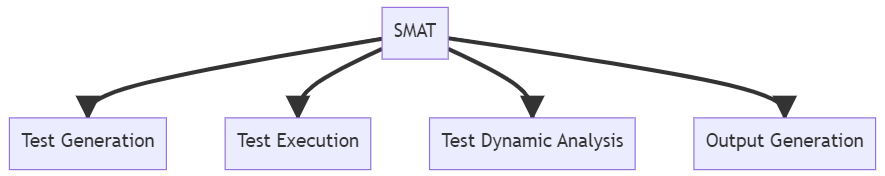
\includegraphics[width=\textwidth]{imagens/macro.png}
    \caption{Diagrama da nova macro-arquitetura proposta para SMAT.}
    \label{fig:macro}
\end{figure}

Cada módulo expõe uma interface pública que permite um ponto único de acesso para as funcionalidades disponíveis e que são então consumidas pela classe principal de controle do sistema responsável por realizar as chamadas na ordem de execução de SMAT. Aspectos utilitários da aplicação, como decodificação da entrada, logging, configuração e a instanciação de objetos foram abstraídos para um módulo separado.

Com o objetivo de aumentar a customização da ferramenta, é possível alterar alguns parâmetros referentes à execução a partir de um arquivo de configuração JSON, cuja estrutura está descrita no Apêndice \ref{apendice-a}.

A fim de mitigar os problemas relacionados ao fraco modelo presente na aplicação, adotamos técnicas de modelagem utilizando o paradigma de orientação a objetos com a finalidade de melhor representar as interações entre as diferentes entidades e serviços envolvidos durante a execução da ferramenta. Nas seções a seguir, discutimos os detalhes e decisões envolvidas no aperfeiçoamento e implementação deste modelo em cada um dos módulos de execução da aplicação.

\subsection{Geração das Suítes de Testes}
A primeira etapa da execução de SMAT consiste da geração de suítes de testes para cada um dos \textit{parents} (de um cenário de \textit{merge}) utilizando ferramentas automáticas de geração de testes unitários como Evosuite e Randoop. Na implementação original de SMAT, um dos principais problemas era o acoplamento entre as etapas de geração, execução e análise dinâmica. Tal acoplamento atingia inclusive a classe de controle, de modo que esta tinha, obrigatoriamente, conhecimento de quais geradores de testes estavam sendo executados conforme mostra o diagrama da Figura \ref{fig:main}, sendo assim difícil adaptar SMAT para usar um conjunto diferente de ferramentas de geração.

\begin{figure}[H]
    \centering
    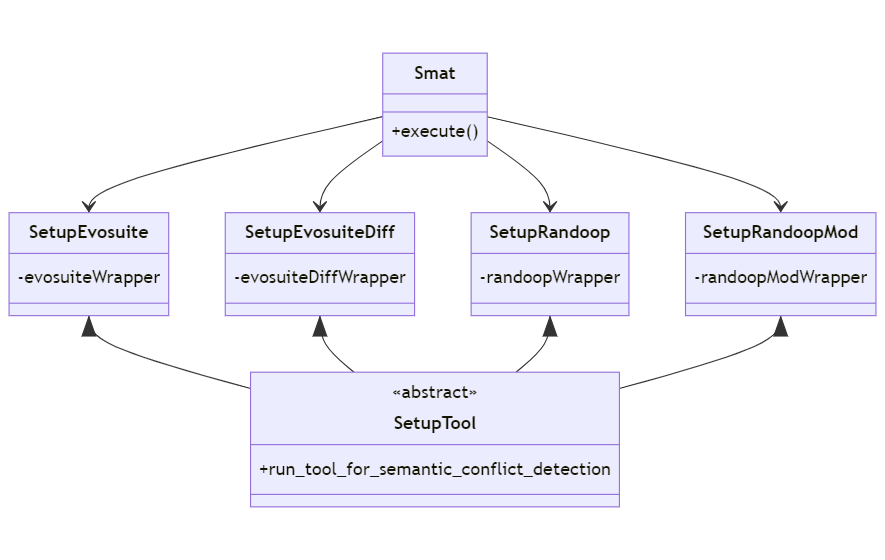
\includegraphics[width=\textwidth]{imagens/main.png}
    \caption{Diagrama de classes simplificado de SMAT. Na implementação original, a classe abstrata SetupTool mistura aspectos de geração, execução e análise dinâmica. Suas subclasses utilizam \textit{wrappers} para realizar a chamada a cada gerador de testes.}
    \label{fig:main}
\end{figure}

Nossa primeira proposta foi a de agrupar todos os conceitos da geração de suíte de testes em um único módulo profundo, que expusesse uma interface simples mas que atendesse às funcionalidades e comportamentos esperados por seus clientes \cite{ousterhout2018philosophy}, chegando então a arquitetura apresentada na Figura \ref{fig:tsg}

\begin{figure}[H]
    \centering
    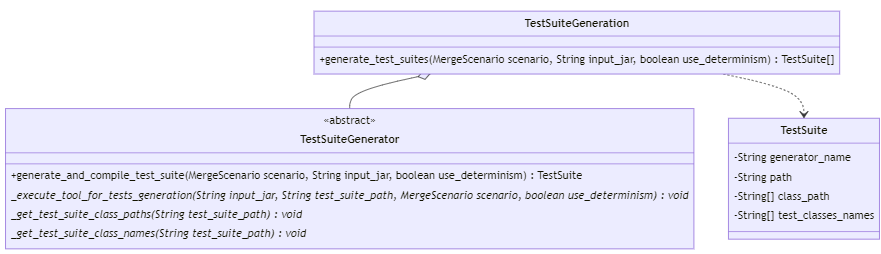
\includegraphics[width=\textwidth]{imagens/tsg.png}
    \caption{Diagrama de classes do módulo de Geração das Suítes de Testes.}
    \label{fig:tsg}
\end{figure}

Neste novo \textit{design}, a classe \textit{TestSuiteGeneration}, que publica a interface deste módulo, expõe um único método que encapsula as sucessivas chamadas a cada um dos geradores de testes implementados. Isso isenta os clientes de conhecerem quais geradores estão sendo executados, simplificando o código da classe de controle e permitindo a possibilidade de customizar os geradores de testes utilizados em tempo de execução, comportamento este implementado a partir de um arquivo de configuração.

Nesta arquitetura, as subclasses de \textit{TestSuiteGenerator} oferecem através de sua interface o método \textit{generate\_and\_compile\_test\_suites}, responsável por realizar a chamada a ferramenta de geração de testes e a posterior compilação do código fonte gerado.

Como cada ferramenta de teste possui características específicas, tais como a invocação da ferramenta, a determinação de quais arquivos gerados devem ser compilados e onde estão localizados, bem como determinar o \textit{classpath} necessário para a compilação da suíte gerada, o método \textit{generate\_and\_compile\_test\_suites} foi implementado utilizando o padrão \textit{template method} \cite{gof}, de modo que o comportamento específico de cada gerador fosse implementado pelas suas subclasses.

Outro ponto de melhoria importante levantado na seção anterior é adicionar a possibilidade de termos determinismo na geração dos testes. Pelo grau de aleatoriedade presente nas ferramentas utilizadas para a geração de testes, atualmente, execuções sucessivas de SMAT podem resultar em resultados diferentes pelas diferenças geradas em cada suíte.

Entretanto, as ferramentas utilizadas disponibilizam funcionalidades que permitem tornar a execução determinística, através do fornecimento de uma \textit{seed} e da alteração em alguns parâmetros durante a invocação da ferramenta, a saber a remoção das restrições de tempo e determinação de novos critérios de parada.

Optamos por abstrair o conceito da geração determinística através de um parâmetro na interface do módulo de geração das suítes, que pode ser configurado pelo usuário final a partir do arquivo de configuração, permitindo dinamicamente habilitar o comportamento determinístico sem que seja necessário alterar o código fonte. Além disto, também é possível customizar a \textit{seed} fornecida às ferramentas através do arquivo de configuração, sendo utilizado um valor padrão caso este não seja informado pelo usuário.

Por último, a introdução da classe \textit{TestSuite} permitiu estruturar os dados das suítes geradas em um objeto, diferentemente da estruturação em n-tuplas utilizada previamente. Embora seja mais verboso, o objeto permite armazenar e acessar com facilidade informações da suíte que serão utilizados em etapas posteriores da execução, como a localização dos arquivos gerados, o gerador utilizado, bem como o nome das classes geradas e o \textit{classpath} dos arquivos compilados.

\subsection{Execução das Suítes de Testes}
Uma vez que a geração das suítes é concluída, é necessário realizar a execução destas suítes em cada uma das versões do \textit{software} presentes no cenário de integração. Para isto, SMAT utiliza-se de um executor de testes, no caso JUnit 4. De forma similar à seção anterior, encapsulamos o comportamento da execução da suíte em um módulo, arquitetado conforme mostra a Figura \ref{fig:tse}.

\begin{figure}
    \centering
    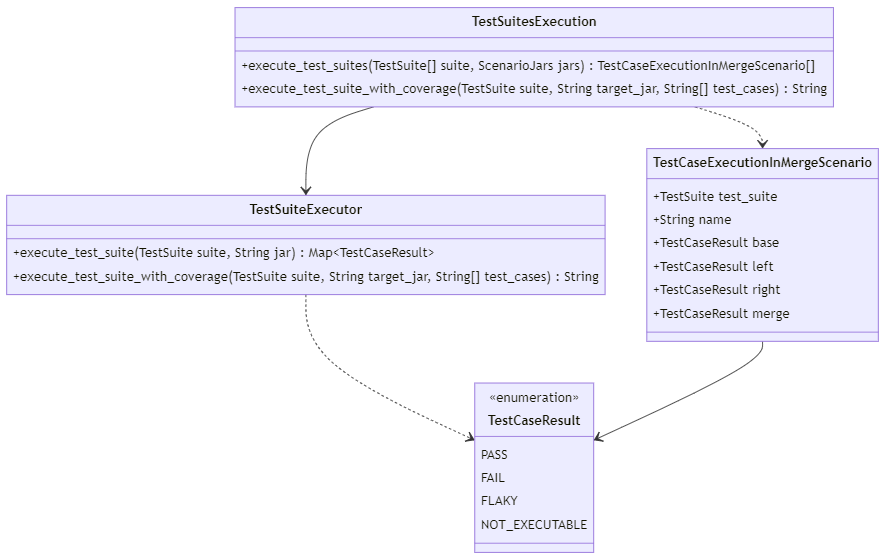
\includegraphics[width=\textwidth]{imagens/tse.png}
    \caption{Diagrama de classes do módulo de Execução das Suítes de Testes.}
    \label{fig:tse}
\end{figure}

Neste design, além de realizar as chamadas às ferramentas que realizam a execução dos testes, a classe \textit{TestSuiteExecutor} também é responsável por realizar a decodificação da saída de \textit{JUnit}, convertendo-a para as representações internas da aplicação, atuando como um Adapter \cite{gof}. Este design permite facilmente substituir o executor de suítes de teste sem ter de se preocupar em eventuais danos a outros aspectos do modelo, contribuindo diretamente com a extensibilidade da ferramenta.
	
Além disso, é importante discutir os diferentes resultados que um caso de teste pode ter em uma determinada execução, para além dos casos triviais: falhar e passar. Como discutido na Seção \ref{smat}, é possível que alguns dos testes gerados previamente possuam comportamento \textit{flaky}, isto é, não possuem resultados consistentes em sucessivas execuções. A fim de tentar detectar este tipo de comportamento, SMAT realiza 3 execuções sucessivas de cada caso de teste marcando-o como \textit{flaky} caso algum resultado seja diferente.

Outro ponto de atenção é na situação em que o caso de teste falha pela ausência de um determinado símbolo que foi introduzido ou removido por alguma modificação em algum dos \textit{commits}. De fato, suponha o trecho de código apresentado na Figura \ref{fig:not_executable} em \textit{merge}, onde a linha 3 indica uma chamada a um método adicionado por \textit{left}. 

\begin{figure}[H]
\begin{minted}{java}
class Aluno {
    public void validarAluno(String email, String cpf) {
        this.validarEmail(email);
        this.validarCpf(cpf);
    }
}
\end{minted}
\caption{Classe de exemplo. O método \textit{validarEmail} foi adicionado por \textit{left}}
\label{fig:not_executable}
\end{figure}

Ao executarmos um caso de teste que exercita o método \textit{validarEmail} em \textit{right} ou \textit{base} seremos surpreendidos com um erro do tipo \textit{NoSuchMethodError}, decorrido da ausência da implementação deste método na classe Aluno nestas versões. Desta forma, embora o teste falhe, esta ocorrência é resultado do fato de o teste sequer ser executável nestas versões do \textit{software}. Ao detectar estes tipos de erros (métodos, atributos e classes faltantes), SMAT classifica tais testes como \textit{NOT\_EXECUTABLE}.

Outra mudança foi a introdução de um novo método que executa a coleta de cobertura de código enquanto realiza a execução dos testes. Na implementação original de SMAT, esta coleta ocorre em todas as chamadas ao módulo de execução, introduzindo uma penalidade considerável em performance, especialmente pela estratégia de executar os testes mais de uma vez. Esta decisão permite que o fluxo secundário de coleta de cobertura seja separado do fluxo primário da execução, resultando em um ganho de performance sem prejuízo semântico ao cliente da aplicação \cite{ousterhout2018philosophy}.

SMAT realiza a coleta de cobertura de código utilizando \textit{Jacoco} \cite{jacoco}. Para isto, é necessário realizar uma instrumentação da versão a ser analisada, para que seja possível detectar quais comandos do código foram executados. Na implementação original, o processo de instrumentação é realizado previamente pelo cliente da classe, que somente então invoca a execução dos testes fornecendo a versão instrumentada.

Esta decisão contribui para que detalhes da implementação da coleta de cobertura estejam expostos ao cliente (a necessidade de realizar um pré-processamento na versão a ser analisada), sinalizando uma quebra do encapsulamento do algoritmo implementado, aumentando a carga cognitiva e complicando a interface do módulo. Em casos extremos, por exemplo, o usuário desta API pode ser surpreendido pelo comportamento do módulo caso forneça uma versão não instrumentada do código, algo que acarretará com que o reporte não seja gerado corretamente.

\cite{ousterhout2018philosophy} afirma que é preferível que um módulo tenha uma interface simples mesmo que isso aumente a complexidade de sua implementação. Baseado neste princípio, decidimos encapsular a lógica de instrumentação da versão a ser analisada no método \textit{execute\_test\_suite\_with\_coverage}. Desta forma, um cliente precisa somente informar a versão na qual deseja realizar a coleta de cobertura, e a implementação será responsável por realizar a instrumentação --- inclusive pulando esta etapa caso uma versão instrumentada já esteja presente --- e realizar a posterior execução e tratamento dos testes.

\subsection{Análise Dinâmica}
Após a execução, é necessário que SMAT realize a análise das execuções dos testes, a fim de verificar se algum deles satisfaz algum dos critérios heurísticos de interferência apresentados na Seção \ref{smat}. Vale ressaltar que, durante a fase de análise, os testes que possuem comportamento \textit{flaky} ou que não são executáveis em alguma versão do \textit{software} são descartados.

Além disso, é importante ressaltar que é possível que exista mudança de comportamento entre diferentes versões do \textit{software} sem que necessariamente ocorra a presença de um conflito. Assim, para fins de estudo, SMAT também computa mudanças de comportamento entre as versões do \textit{software} verificando pares de versões que possuem resultados diferentes para um mesmo caso de teste.

Na implementação original, tanto a verificação de conflitos quanto de mudanças de comportamento são realizadas por uma única classe\footnote{\href{https://github.com/spgroup/SMAT/blob/ae33ccdc49/nimrod/setup\_tools/behaviour\_check.py}{https://github.com/spgroup/SMAT/blob/ae33ccdc49/nimrod/setup\_tools/behaviour\_check.py}}. Nesta versão, os casos de testes são separados em diferentes conjuntos: os que passaram, os que falharam e os que possuem comportamento \textit{flaky} ou que não foram executados. As verificações são realizadas então utilizando operações entre estes diferentes conjuntos, o que torna difícil a compreensão de como cada critério é definido apenas pela leitura do código.

Além disso, a ausência do uso de objetos e pela estratégia de dividir os casos de testes em diferentes conjuntos polui a interface dos métodos, que acabam tendo elevado número de parâmetros resultando em um \textit{code smell} \cite{fowler2018refactoring}. A ausência de um modelo orientado a objetos também resulta em um uso abusivo de tipos primitivos, que acabam por não expressar de forma clara o comportamento e as relações entre os diferentes componentes do \textit{software}.

Neste sentido, nosso primeiro passo é construir um modelo que consiga refletir a relação existente entre a execução de um caso de teste em um determinado cenário e se ele satisfaz ou não um determinado critério heurístico da ferramenta. Para modelar esta relação bem como os possíveis múltiplos critérios existentes para a detecção de conflitos, encapsulamos tal comportamento na interface \textit{SemanticConflictCriteria}. Na situação de uma execução de um caso de teste satisfazer algum destes critérios, estes são encapsulados em uma instância da classe \textit{SemanticConflict}. Essa visão parcial do modelo de análise dinâmica está representado no diagrama da Figura \ref{fig:criteria}.

\begin{figure}[H]
    \centering
    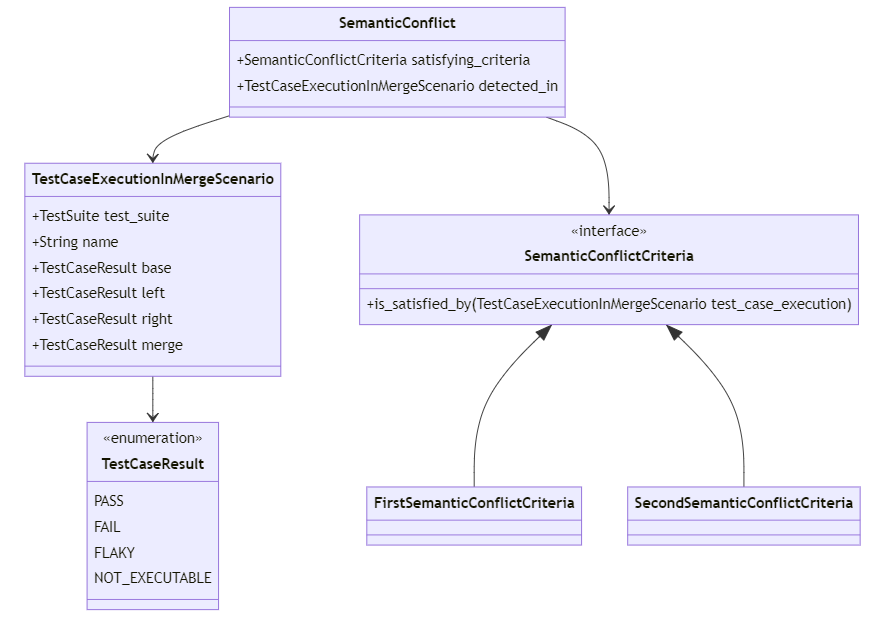
\includegraphics[width=\textwidth]{imagens/criteria.png}
    \caption{Diagrama de classes da estruturação da análise de conflitos semânticos.}
    \label{fig:criteria}
\end{figure}

Com este modelo, a implementação dos critérios de conflitos tem sua implementação drasticamente simplificada, se assemelhando bastante a sua descrição em linguagem natural, conforme mostra a Figura \ref{fig:criteria-python} que ilustra a implementação para o segundo critério apresentado na seção \ref{smat}

\begin{figure}[H]
\begin{minted}[fontsize=\small]{python}
class SecondSemanticConflictCriteria(SemanticConflictCriteria):
  def is_satisfied_by(self, test_case_execution):
    fails_in_base_and_both_parents_but_passes_in_merge = \
        test_case_execution.base == TestCaseResult.FAIL \
        and test_case_execution.left == TestCaseResult.FAIL \
        and test_case_execution.right == TestCaseResult.FAIL \
        and test_case_execution.merge == TestCaseResult.PASS
    passes_in_base_and_both_parents_but_fails_in_merge = \
        test_case_execution.base == TestCaseResult.PASS \
        and test_case_execution.left == TestCaseResult.PASS \
        and test_case_execution.right == TestCaseResult.PASS \
        and test_case_execution.merge == TestCaseResult.FAIL
    return fails_in_base_and_both_parents_but_passes_in_merge or \
    passes_in_base_and_both_parents_but_fails_in_merge
\end{minted}
\caption{Implementação da detecção do segundo critério de conflitos}
\label{fig:criteria-python}
\end{figure}

Uma estratégia similar pode ser utilizada para identificar as mudanças de comportamento entre diferentes versões do \textit{software}. De fato, o modelo resultante é semelhante, conforme mostra a Figura \ref{fig:bc}.

\begin{figure}[H]
    \centering
    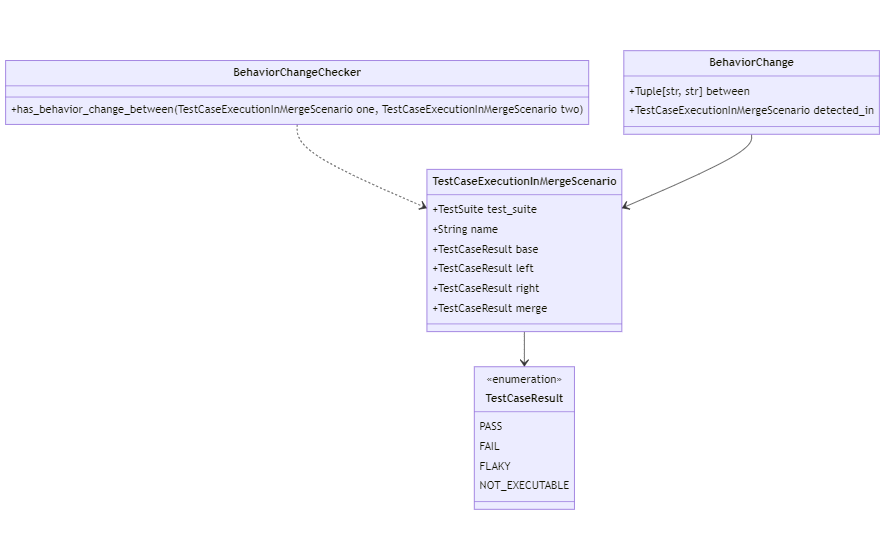
\includegraphics[width=\textwidth]{imagens/bc.png}
    \caption{Diagrama de classes da estruturação da análise de mudanças de comportamento.}
    \label{fig:bc}
\end{figure}

A fim de simplificar o consumo por parte de seus clientes, as implementações do módulo de Análise Dinâmica foram agrupadas em uma Fachada \cite{gof}, que agrupa as funcionalidades principais fornecidas pelo módulo. Desta forma, uma visão geral do módulo é apresentada na Figura \ref{fig:da}.

\begin{figure}[H]
    \centering
    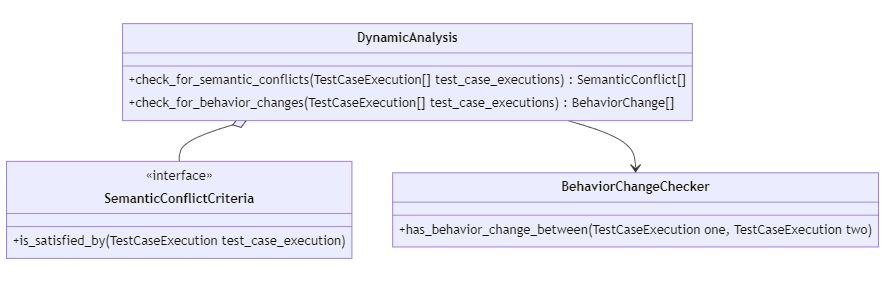
\includegraphics[width=\textwidth]{imagens/da.png}
    \caption{Diagrama de classes em alto nível do módulo de análise dinâmica.}
    \label{fig:da}
\end{figure}

\subsection{Geração de relatórios}

Com as análises finalizadas, a última etapa da execução de SMAT consiste em construir relatórios com os dados coletados para que estes possam ser consumidos e analisados pelo usuário ou por outras ferramentas.

A ferramenta permite a confecção de 3 tipos de relatórios: um com informações a respeito dos conflitos semânticos detectados, outro possuindo informações a respeito das mudanças de comportamento  observadas entre as diferentes versões do cenário e um último reporte contendo informações a respeito das suítes de testes geradas. A Figura \ref{fig:relatorios} mostra a estrutura de cada um dos relatórios gerados.

\begin{figure}[H]
    \centering
    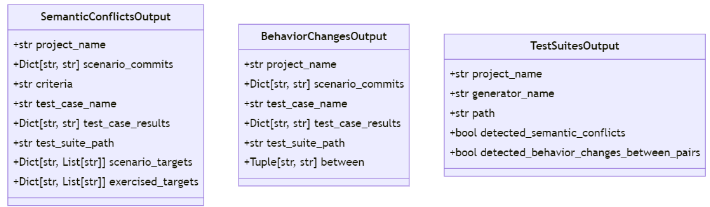
\includegraphics[width=\textwidth]{imagens/relatorios.png}
    \caption{Estrutura de cada um dos relatórios gerados. Cada relatório é composto de uma lista de instâncias destas classes.}
    \label{fig:relatorios}
\end{figure}

Seguindo a mesma estratégia utilizada nas outras seções, decidimos por isolar a geração de relatórios em um módulo na aplicação. Este módulo possui uma classe abstrata \textit{OutputGenerator} responsável por realizar a geração de um relatório. Embora na versão original de SMAT os relatórios fossem gerados em formato CSV, optamos por utilizar JSON em nossa implementação, pela possibilidade de representar mais facilmente estruturas como dicionários e listas.

Como cada relatório possui uma estratégia diferente para sua geração, consultando dados diferentes e aplicando processamentos específicos, cada subclasse deve sobrescrever o método abstrato \textit{\_generate\_report\_data} introduzindo o comportamento necessário para a confecção do relatório, resultando assim em mais uma aplicação do padrão \textit{template method} \cite{gof}. A Figura \ref{fig:output} apresenta a arquitetura do módulo de geração de reportes.

\begin{figure}[H]
    \centering
    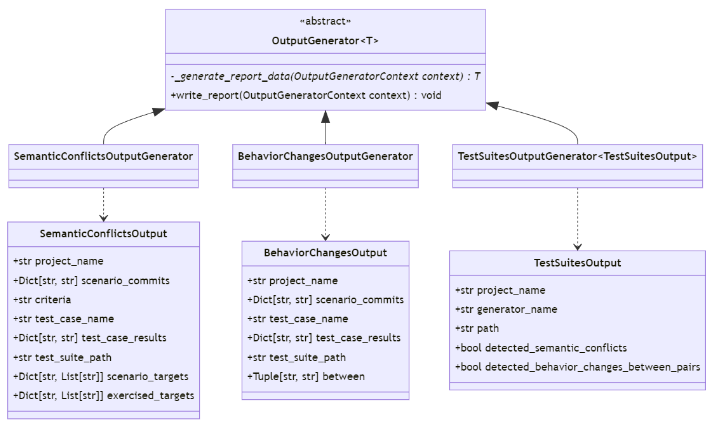
\includegraphics[width=0.8\textwidth]{imagens/output.png}
    \caption{Diagrama de classes do módulo de geração de relatórios}
    \label{fig:output}
\end{figure}

Um aspecto importante a ser considerado neste módulo é a necessidade de consultar valores computados em diferentes etapas da execução. Por exemplo, os reportes de conflitos semânticos necessitam de informações obtidas durante a etapa de análise dinâmica, enquanto o reporte de suítes de teste consulta informações da geração de suítes e de análise dinâmica.

A fim de preservar uma interface comum para os diferentes geradores de relatório, o que simplifica a consumação da classe pelos seus clientes, decidimos por ter como parâmetro da geração de relatório as diferentes entidades das etapas anteriores. Entretanto, para evitar o \textit{code smell Long Parameter List} \cite{fowler2018refactoring}, quando um método possui diversos parâmetros, decidimos por encapsular estes parâmetros em um único objeto, utilizando a técnica de \textit{Introduce Parameter Object} \cite{fowler2018refactoring}.

\begin{figure}[H]
    \centering
    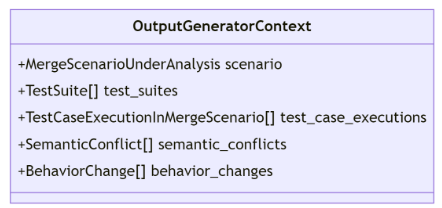
\includegraphics{imagens/ogc.png}
    \caption{Diagrama do objeto \textit{OutputGeneratorContext}, que guarda as diversas informações a serem consultadas durante a geração de um relatório.}
    \label{fig:ogc}
\end{figure}

\subsection{Documentação e gerência do projeto}
A fim de melhorar a manutenibilidade do projeto, iniciamos a produção de documentações relevantes. A fim de documentar as diferentes decisões arquiteturais tomadas ao longo do projeto, adicionamos um documento de arquitetura ao projeto, que possui diagramas que discutem em alto nível as decisões, implicações e \textit{trade-offs} levados em consideração durante a fase de projeto.

Do ponto de vista de gerenciamento do projeto, a principal preocupação foi a de permitir o aumento da utilização de ferramentas de verificação estática do código a fim de encontrar possíveis defeitos ainda em tempo de compilação. Neste sentido, foram adicionadas anotações de tipos estáticos em todas as novas implementações, bem como adicionadas verificações destes tipos a esteira de integração contínua do projeto.

\section{Discussão e Trabalhos Futuros}
SMAT é uma ferramenta que tenta encontrar conflitos semânticos em um cenário de integração de código a partir da detecção automática de mudanças de comportamento utilizando geração de testes automáticos. Durante este trabalho, tivemos a oportunidade de revisitar, reestruturar e aperfeiçoar diversos aspectos desta ferramenta. Nesta seção, discutimos os resultados dessas modificações e como elas podem contribuir na evolução e manutenção do produto, bem como apresentamos possibilidades de trabalhos futuros.

Em primeiro lugar, é importante destacar que a nova implementação de SMAT permitiu que a ferramenta atingisse um maior nível de configurabilidade, de forma que diversos aspectos possam ser configurados diretamente em tempo de execução, como definir quais serão as ferramentas utilizadas durante a etapa de geração de testes, bem como customizar parâmetros relevantes para a execução como o tempo disponível para a busca e definir quais reportes serão elaborados na etapa de geração de saída.

Outro aperfeiçoamento introduzido na ferramenta foi a possibilidade de execuções determinísticas da ferramenta, permitindo que execuções sucessivas com a mesma entrada tenham sempre o mesmo resultado. Este aperfeiçoamento facilita a reprodutibilidade dos experimentos realizados com a ferramenta, um aspecto que foi observado como um dos principais pontos de melhoria da ferramenta.

Do ponto de vista arquitetural, a ferramenta possui agora um modelo que facilita o entendimento, evolução e manutenção do \textit{software}. Através de um maior entendimento de aspectos importantes do domínio da ferramenta, foi possível introduzir abstrações que permitissem estruturar as diversas entidades da aplicação e como estas se relacionam durante a execução da ferramenta.

Além disso, a nova arquitetura dos módulos facilita a extensibilidade do \textit{software} sem que seja necessário modificar componentes já existentes. Em todos os contextos da aplicação, adicionar novas ferramentas ou funcionalidades se limita a implementar uma única subclasse. É o caso na adição de novos geradores de testes, novos critérios heurísticos para detecção de conflitos e novos geradores de relatórios.

Vale ressaltar também que a remoção do acoplamento entre as etapas de geração, execução e análise dinâmica permite agora que um desenvolvedor responsável por uma tarefa que envolva apenas uma dessas etapas não tenha de se preocupar ou conhecer detalhes da implementação das etapas adjacentes, diminuindo a carga cognitiva exigida e reduzindo a probabilidade do surgimento de defeitos.

A introdução de novas interfaces de entrada e saída para os clientes da ferramenta utilizando JSON também contribuiu para facilitar o uso da ferramenta. Ao termos a possibilidade de representar estruturas complexas exigidas pela ferramenta de maneira trivial, sem ser necessário a substituição de caracteres ou utilização de separadores customizados, eliminamos um trabalho considerável do cliente em construir uma entrada que adote as notações utilizadas bem como seja capaz de converter a saída para sua representação interna.

A introdução de uma interface que permitisse que uma mesma execução de SMAT fosse capaz de buscar conflitos semânticos em mais de um alvo, trouxe um ganho de performance considerável, especialmente nos cenários onde vários alvos precisam ser investigados. Além disso, a estratégia introduzida para detectar quais destes alvos foram executados durante um conflito, permitiu também resolver uma das fontes de falsos positivos discutidas pelos autores em trabalhos anteriores. 

Como trabalhos teóricos futuros, temos como principal horizonte a expansão de SMAT para que ela seja capaz de atender outros projetos para além da linguagem Java. Vale ressaltar aqui que tal expansão depende da existência de ferramentas que sejam capazes de realizar a geração de testes automáticos para diferentes linguagens, e que estas ferramentas ainda estão em desenvolvimento dentro da literatura.	

A nível de implementação, uma das principais necessidades consiste no aumento da cobertura de testes automatizados da aplicação. É importante ressaltar que com o advento das execuções determinísticas implementadas neste trabalho, é possível construir valiosas suítes de testes de integração que podem, com baixo custo de desenvolvimento, serem capazes de encontrar com facilidade possíveis regressões em tarefas de desenvolvimento futuras.

Além disso, o isolamento da execução dos geradores de suítes de testes permite explorar possibilidades de execução da geração em paralelo. Embora uma análise menos criteriosa aponte para a possibilidade de um ganho de performance, é necessário considerar como este comportamento influenciaria a qualidade e o tempo disponível para a geração de cada uma das suítes, especialmente quando utilizando a busca exploratória limitada por tempo.

Por último, contribuições na documentação da ferramenta, na remoção de trechos de código não mais utilizados e na implementação de uma política de refatoração contínua são também possíveis áreas de interesse para trabalhos futuros.

\bibliographystyle{sbc}
\bibliography{sbc-template}

\newpage

\appendix
\section{Estrutura do arquivo de configuração de SMAT} \label{apendice-a}
SMAT permite que o usuário customize alguns aspectos de sua execução. Estas modificações podem ser realizadas editando o arquivo \textit{nimrod/tests/env-config.json}. Este documento discute as opções disponíveis para customização.

\subsection{Geral}
As propriedades a seguir se referem a aspectos gerais da execução de SMAT.

\subsubsection{java\_home}
Por padrão, SMAT utilizará a variável de ambiente \textit{JAVA\_HOME} para popular o caminho de instalação do Java. Entretanto, é possível sobrescrever esse valor configurando a variável \textit{java\_home} no arquivo de configuração.

\subsubsection{maven\_home}
Por padrão, SMAT utilizará a variável de ambiente \textit{MAVEN\_HOME} ou MVN\_HOME para popular o caminho de instalação do Maven. Entretanto, é possível sobrescrever esse valor configurando a variável \textit{maven\_home} no arquivo de configuração.

\subsubsection{logger\_level}
Esta propriedade permite alterar o nível mínimo de mensagens que serão exibidas pela CLI. O valor padrão é \textit{INFO}, podendo ser alterada para: \textit{CRITICAL}, \textit{ERROR}, \textit{WARNING} ou \textit{DEBUG}.

\subsubsection{input\_path}
Esta propriedade contém o caminho absoluto para o arquivo JSON que contém a descrição dos cenários a serem analisados pela ferramenta.

\subsection{Geração de Suítes de Teste}
As propriedades a seguir estão relacionadas com aspectos da etapa de Geração de Suítes de Teste.

\subsubsection{test\_suite\_generators}
Um \textit{array} com o nome das ferramentas a serem utilizados durante a etapa de geração. Se não for informado, todos os geradores implementados serão utilizados. Valores válidos são: \textit{randoop, randoop-modified, evosuite} e \textit{evosuite-differential}.

\subsubsection{test\_suite\_generation\_search\_budget}
Permite customizar o tempo em segundos disponível para cada gerador durante a etapa de Geração de Suítes de Testes. O valor padrão é de 300 segundos. Observe que esta opção será ignorada se a geração de testes for determinística.

\subsubsection{generate\_deterministic\_test\_suites}
Se configurada para \textit{true}, SMAT utilizará versões determinísticas de seus gerados, i.e., as suítes geradas serão sempre as mesmas independente de quantas vezes a ferramenta seja executada.

\subsection{Output Generation}
As propriedades a seguir estão relacionadas com aspectos da etapa de Geração de Reportes.

\subsubsection{output\_generators}
Um \textit{array} contendo os relatórios que devem ser escritos durante a etapa de geração de relatórios. Se não for informada, todos os relatórios implementados serão gerados. Valores válidos são: \textit{behavior\_changes, semantic\_conflicts, test\_suites}.

\end{document}
